\documentclass[12pt]{jsarticle}

\setcounter{secnumdepth}{3}
%\setcounter{figure}{1}
\usepackage[dvipdfmx]{graphicx}
\usepackage{amsmath}
\usepackage{float}
\usepackage{bm}
\usepackage{listings}

\pagestyle{myheadings}

\usepackage{titlesec}
\usepackage{cases}
\titleformat*{\section}{\large}
\titleformat*{\subsection}{\normalsize\bf}
\renewcommand{\lstlistingname}{ソースコード}
\lstset{
  basicstyle={\ttfamily},
  language=Python,
  identifierstyle={\small},
  commentstyle={\smallitshape},
  keywordstyle={\small\bfseries},
  ndkeywordstyle={\small},
  stringstyle={\small\ttfamily},
  frame={tb},
  breaklines=true,
  columns=[l]{fullflexible},
  numbers=left,
  xrightmargin=0zw,
  xleftmargin=3zw,
  numberstyle={\scriptsize},
  stepnumber=1,
  numbersep=1zw,
  lineskip=-0.5ex
}
\begin{document}
\section{目的}
状態フィードバック制御を行うためには全状態量をフィードバックする必要がある.しかしセンサの不足などによって実際に測定できない状態量が存在する場合には,オブザーバ(状態観測器)を用いて状態量を推定し,フィードバック制御に利用する.本実験では,台車の位置制御実験を通じて,オブザーバによる状態フィードバック制御について理解を深める.
\section{実験装置の概要}
制御系の構成の概要を図\ref{B2-1}に示す.制御目的は,レール上の台車を目的位置に移動させ,停止させることである.モータドライバに電圧を加えるとモータが回転し,ベルトで台車を移動させる.台車の変位$y$はポテンシャルメータで電圧値として検出され,A/D変換器を介して制御用計算機に送られる.計算機でモータドライバへの指令電圧$u$が計算され,D/A変換を介して出力される.
\begin{figure}[H]
  \begin{center}
    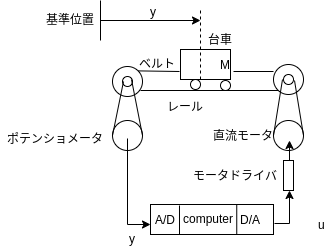
\includegraphics[clip,width=7.0cm]{../img/B2-1.png}
    \caption{実験書の記述}%TODO
    \label{B2-1}
  \end{center}
\end{figure}
\section{原理}
\subsection{数式モデル}
モータの回転による力$T_u$を入力,台車の変位$y$を出力としたとき,運動方程式は次のようになる.
\begin{equation}
  \label{Equation-B2-1}
  M\ddot{y} + F\dot{y} = T_u
\end{equation}
$M$は台車の等価質量,$F$はレールとの間の摩擦係数である.$T_u$はパソコンからの指令電圧$u$に比例する.すなわち,$T_u=\alpha u$.ただし,$\alpha = 20.09{\rm [N/V]}$.\\
状態変数を${\bm x}=\left[\begin{array}{cc}x_1 & x_2\end{array}\right]^T = \left[\begin{array}{cc}y & \dot{y}\end{array}\right]^T$とおくと,次の状態方程式が得られる.
\begin{eqnarray}
  \label{Equation-B2-2}
  \dot{\bm x} &=& \left[\begin{array}{cc}0& 1\\0& -F/M\end{array}\right] {\bm x} + \left[\begin{array}{c}0\\\alpha/M\end{array}\right] u \\ \nonumber
  y &=& \left[\begin{array}{cc}1 &0\end{array}\right] {\bm x}
\end{eqnarray}
ただし$T$はベクトルの転置を意味する.
\subsection{未知パラメータの同定}
状態フィードバック制御系を構成するためには,式(\ref{Equation-B2-2})の中の動特性パラメータがわかっている必要がある.システムのステップ応答より$F$と$M$を同定することができる.式(\ref{Equation-B2-2})より,台車に一定の力を入力すると,台車は一方向に走りっぱなしになる.そこで,次の出力フィードバックをかける.

\begin{equation}
  \label{Equation-B2-3}
  u = h(r - y)
\end{equation}
ただし,$r$は台車の目標ステップ変位,$h$はフィードバックゲイン定数である.すると,$r$から$y$までの伝達関数は式(\ref{Equation-B2-4})となる.この系の応答波形は$h$の値によって変わる.
\begin{equation}
  \label{Equation-B2-4}
  G(s) = \frac{Y(s)}{R(s)} = \frac{b_0}{s^2+a_1s+a_0}\;\;\;\;(a_1 =F/M,a_0=b_0=\alpha h /M)
\end{equation}
したがって,$a_0$,$a_1$が求まれば,$F$,$M$が計算できる.$a_0$,$a_1$の求め方はステップ応答を用いた二次遅れ系のパラメータ同定,同定結果の検証の節を参照せよ.
\subsection{制御系の構成}
式(\ref{Equation-B2-2})に対し以下のように状態フィードバック制御系を構成する.
\begin{eqnarray}
  \label{Equation-B2-5}
  \dot{\bm x}(t) &=& {\bm A}{\bm x}(t) + {\bm b}u(t) \\
  \label{Equation-B2-6}
  y(t) &=& {\bm c}{\bm x}(t)
\end{eqnarray}
ただし,
\begin{equation}
  \label{Equation-B2-7}
  {\bm A} = \left[\begin{array}{cc}0&1\\ 0&-F/M\end{array}\right], {\bm b} = \left[\begin{array}{c}0\\ \alpha/M\end{array}\right], {\bm c} = [\begin{array}{cc}1&0\end{array}]
\end{equation}
\begin{equation}
  \label{Equation-B2-8}
  u(t) = -{\bm f}{\bm x}(t) = [\begin{array}{cc}-f_1&-f_2\end{array}][\begin{array}{cc}x_1(t)&x_2(t)\end{array}]^T
\end{equation}
本実験では二つの状態,すなわち台車位置$x_1(t)$と台車速度$x_2(t)$のうちセンサで検出できるのは$x_1(t)$だけである.したがって,状態フィードバックを行うためには,オブザーバによる状態の推定値を用いる必要がある.そこで,式(\ref{Equation-B2-6})のプラントに対し,次の同一次元オブザーバを構成する.
\begin{eqnarray}
  \label{Equation-B2-9}
  \dot{\hat{\bm x}}(t) &=& {\bm A} \hat{\bm x} + {\bm b}u(t) + {\bm k}(y(t) - \hat{y}(t)) \\
  \label{Equation-B2-10}
  \hat{y}(t) &=& {\bm c}\hat{\bm x}(t)
\end{eqnarray}
$\hat{\bm x}(t)$は状態${\bm x}(t)$の推定状態量である.これらより,台車を初期位置から目標位置に移動させる制御は次の入力を用いることによって達成される.
\begin{equation}
  \label{Equation-B2-11}
  u(t) = -{\bm f} \hat{\bm x}(t) = \left[\begin{array}{cc}-f_1&-f_2\end{array}\right]\left[\begin{array}{cc}(\hat{x}_1(t)-y_r)&\hat{x}_2(t)\end{array}\right]^T
\end{equation}
ただし,$y_r$は台車の目標位置である.制御系全体の構成を図\ref{Fig2-2}に示す.
\begin{figure}[tb]
  \begin{center}
    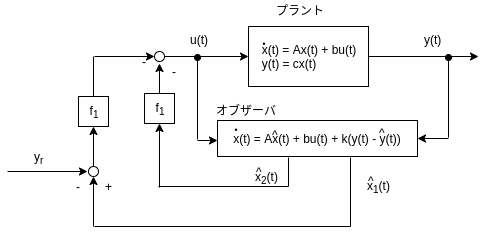
\includegraphics[clip,width=7.0cm]{../img/B2-2.png}
    \caption{実験書の記述}%TODO
    \label{B2-2}
  \end{center}
\end{figure}
\subsection{ステップ応答を用いた二次遅れ系のパラメータ同定}
二次遅れ系の伝達関数が次式のように与えられているとする.
\begin{equation}
  \label{Equation-2-B1}
  G(s) = \frac{b_0}{s^2+a_1s+a_0}
\end{equation}
また,ステップ入力$r$に対する応答が図\ref{Fig2-B1}のような振動的な波形($G(s)$が複素極をもつ)になったとする.この応答波形において,最初のピーク値は,$t=0$以外に最初に$dy(t)/dt = 0$となる時点で生じる.このことを利用すれば,式(\ref{Equation-2-B2})の関係が得られる.
\begin{figure}[tb]
  \begin{center}
    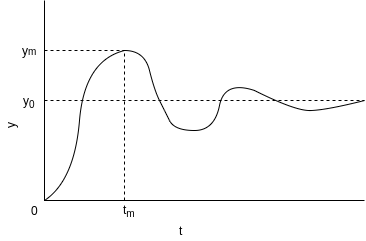
\includegraphics[clip,width=7.0cm]{../img/2-B1.png}
    \caption{実験書の記述}%TODO
    \label{Fig2-B1}
  \end{center}
\end{figure}
\begin{equation}
  \label{Equation-2-B2}
  a_1 = -\frac{1}{t_m}2{\rm ln}(y_m/y_0 -1),  a_0 = \frac{\pi^2}{t_m^2}+\frac{a_1^2}{4}
\end{equation}
ただし,$y_m$は応答波形の最初のピーク値,$t_m$はその時間である.$y_0$は応答の整定値である.また,$b_0=a_0y_0/r$となる.したがって,図\ref{Fig2-B2}を用いて$G(s)$のパラメータが計算できる.
\subsection{同定結果の検証}
式(\ref{Equation-B2-4})より,
\begin{equation}
  \label{Equation-2-B3}
  Y(s) = \frac{b_0}{s^2+a_1 s + a_0}R(s),    a_1=\frac{F}{M}, a_0=\frac{\alpha h}{M}, b_0=\frac{a_0 y_0}{r}
\end{equation}
である.同定の過程で$R(s)=r/s$としたので,
\begin{equation}
  \label{Equation-2-B4}
  Y(s) = \frac{b_0}{s^2+a_1 s + a_0} R(s) = \frac{\frac{y_0 a_0}{r}}{s^2+a_1s+a_0}\frac{r}{s} = \frac{a_0}{s^2+a_1s+a_0}\frac{1}{s}y_0
\end{equation}
と表せる.ここで
\begin{equation}
  \label{Equation-2-B5}
  \frac{a_0}{s^2+a_1s+a_0} = \frac{\omega_n^2}{s^2+2\zeta \omega_ns + \omega_n^2}
\end{equation}
と表現しなおすと,式(\ref{Equation-2-B4})は以下のように書ける.
\begin{equation}
  \label{Equation-2-B6}
  Y(s) = \frac{\omega_n^2}{s^2+2\zeta \omega_n s + \omega_n^2}\frac{1}{s}y_0 = y_0(\frac{1}{s} - \frac{s+2\zeta \omega_n}{s^2 + 2\zeta \omega_n s + \omega_n^2})
\end{equation}
これを逆ラプラス変換すると,
\begin{equation}
  \label{Equation-2-B7}
  y(t) = y_0 \left(1 - \frac{1}{\sqrt{1-\zeta^2}}e^{-\beta t} {\rm cos}(\gamma t - \delta)\right)
\end{equation}
となる.ただし,$\beta=\zeta \omega_n$,$\gamma =\omega_n \sqrt{1-\zeta^2}$,$\delta={\rm tan}^{-1}(\frac{\zeta}{\sqrt{1-\zeta^2}})$である.$\omega_n=\sqrt{a_0}$,$\zeta=\frac{a_1}{2\sqrt{a_0}}$であることに注意して,上式に各自の求めたパラメータを代入すれば時間応答が得られる.この同定結果に基づく時間応答に基づく時間応答と実験結果を比較し,同定パラメータが妥当か検証する必要がある.
\subsection{状態フィードバック制御系の設計}
離散時間プラントが次式で与えられているとする.
\begin{eqnarray}
  \label{Equation-2-B8}
  \begin{cases}
  {\bm x}(k+1) = {\bm P}{\bm x}(k) + {\bm q}u(k) & \\
  y(k) = {\bm c}{\bm x}(k) &
  \end{cases}
\end{eqnarray}
この系が可制御なら,状態フィードバックにより極配置できる.
$u(k)=-{\bm f}{\bm x}(k)$とすると,閉ループ系は
\begin{equation}
  \label{Equation-2-B9}
  {\bm x}(k+1) = ({\bm P} - {\bm q}{\bm f}){\bm x}(k)
\end{equation}
となる.$\bm f$はフィードバック係数ベクトルである.$({\bm P}-{\bm q}{\bm f})$の固有値を単位円内の希望の位置に配置するように$\bm f$を決めればよい.特性方程式の係数比較によって$\bm f$を求めることができる.その手順を以下に示す.
\begin{description}
  \item[(1)] 希望固有値を$\lambda_1$,$\lambda_2$とし,係数ベクトルを${\bm f}=\left[\begin{array}{cc}f_1&f_2\end{array}\right]$とする.
  \item[(2)] $({\bm P}-{\bm q}{\bm f})$の特性方程式を計算する.
    \begin{equation}
      \label{Equation-2-B10}
      |\lambda {\bm I} - ({\bm P}-{\bm q}{\bm f})| = \lambda^2 + \mu_1 \lambda + \mu_2 = 0
    \end{equation}
  \item[(3)] 希望固有値の特性方程式を計算する.
    \begin{equation}
      \label{Equation-2-B11}
      (\lambda - \lambda_1)(\lambda - \lambda_2) = \lambda^2 + \theta_1 \lambda + \theta_2 = 0
    \end{equation}
  \item[(4)] 式(\ref{Equation-2-B10})と式(\ref{Equation-2-B11})の係数を比較することにより次の関係を得る.
    \begin{equation}
      \label{Equation-2-B12}
      \mu_1 = \theta_1,  \mu_2 = \theta_2
    \end{equation}
\end{description}
これを解くことにより$f_1$,$f_2$を求める.
状態${\bm x}(k)$が直接観測できない場合には,オブザーバによる推定値$\hat{\bm x}(k)$を用いる.すなわち,$u(k)=-{\bm f}{\bm x}(k)$の代わりに,$u(k)=-{\bm f}\hat{\bm x}(k)$とする.
\section{実験方法}
\begin{description}
  \item[注1] 実験は各自の設定および計算結果に基づいて一人ずつ行う.
  \item[注2] 台車がレール上の制限位置を越えたり,正しく動作しない場合には,モータスイッチを切り,手で台車を初期位置に戻し,リセットボタンを押す.なお,右方向が正の方向である.
\end{description}
\subsection{同定実験(一週目)}
\begin{description}
  \item[(1)] 台車をレールの中央より左側にセットした.
 \item[(2)] 計算機の電源を入れた.ログイン画面でユーザ名:root,パスワード:keisokuを入力してログインした.次にターミナルを開いて,ディレクトリuser3に移動した.user3に移動するためには次のコマンドを入力した.
\begin{center}
  \# cd user3
\end{center}
  \item[(3)] douteiを実行した.
\begin{center}
  \# ./doutei
\end{center}
  画面の指示にしたがって,式(\ref{Equation-B2-3})の台車の目標ステップ変位$r$とフィードバックゲイン$h$を入力した.$r$は0.4[m]を選んだ.$h$は10とした.画面の指示にしたがって,時間-台車位置のデータを出力し,ファイルに保存した.
  \item[(4)] 時間-台車位置のデータを使って,台車のステップ応答波形を作成した.
\end{description}
\subsection{計算(二週目)}
\begin{description}
  \item[(1)] 同定実験で得られた台車のステップ応答波形より必要な情報を読み取り,式(\ref{Equation-B2-2})の$a_0$と$a_1$,さらに$F$と$M$を算出した.
  \item[(2)] (1)で得られた未知パラメータ$F$と$M$を用いて,式(\ref{Equation-B2-2})のモデルを計算した.得られた制御対象のパラメータから応答波形をシミュレーションし,同定実験結果と比較した.実験結果をより正確に再現するような$F$と$M$の値を再計算して求め,以下の計算に用いよ.
  \item[(3)] 状態フィードバック係数ベクトルを決めた.
  \item[(4)] オブザーバの各係数を計算した.
  \item[(5)] 設計が妥当か検討した.
\end{description}
\subsection{制御実験(三週目)}
\begin{description}
  \item[(1)] 台車をレールの中央より左側にセットした.
  \item[(2)] 台車の初期位置およびレールの長さの制限を考慮し,目標位置$y_r$を決めた.
  \item[(3)] ディレクトリuser3に移動してcntlを実行させた.
\begin{center}
  \# ./cntl
\end{center}
画面の指示に従って,各パラメータを順番に入力してスタートさせた.画面の指示にしたがって,データをファイルに保存した.ファイル名には学籍番号を付けた.
  \item[(4)] 時間の許す限り,パラメータ等を見直して再実験してもよい.
  \item[(5)] 実験結果をグラフに整理した.台車位置,入力電圧,オブザーバの位置,速度の推定の時間遷移についてまとめた.
\end{description}
\section{実験結果}
同定実験の結果は図\ref{Figure-doutei}のようになった.
\begin{figure}[tb]
  \begin{center}
    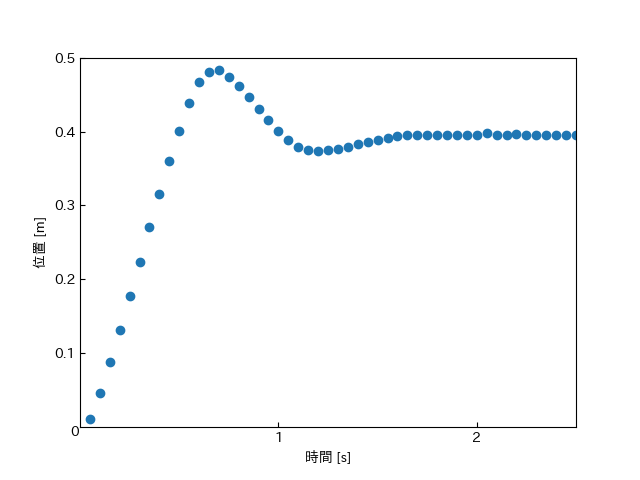
\includegraphics[clip,width=7.0cm]{../img/doutei.png}
    \caption{同定実験により得られたグラフ}
    \label{Figure-doutei}
  \end{center}
\end{figure}
定常値$y_0$,最大値$y_m$はそれぞれ$y_0=0.394675{\rm [m]}$,$y_m=0.482656{\rm [m]}$だった.
また,行き過ぎ時間$t_m$は$t_m=0.70{\rm [s]}$だった.
二次遅れ系の伝達関数を式(\ref{Equation-2-B1})として考えると,ステップ応答の結果から,$a_0$,$a_1$は次のように求められる.
\begin{eqnarray}
  \label{StepResponse_calculate_a1}
  a_1 &=& -\frac{1}{t_m}2{\rm ln}(y_m/y_0 - 1) \\
      &=& 4.2884 \nonumber
\end{eqnarray}
\begin{eqnarray}
  \label{StepResponse_calculate_a0}
  a_0 &=& \frac{\pi^2}{t_m^2} + \frac{a_1^2}{4} \\
      &=& 24.73 \nonumber
\end{eqnarray}
台車の等価質量$M$,レールとの間の摩擦係数$F$は次のように求められる.
\begin{eqnarray}
  \label{StepResponse_calculate_M}
  M &=& \frac{\alpha h}{a_0} \\
    &=& 8.12057 \nonumber
\end{eqnarray}
\begin{eqnarray}
  \label{StepResponse_calculate_F}
  F &=& M a_1\\
    &=& 34.82427 \nonumber
\end{eqnarray}
また,時間応答に用いるパラメータは次のように求められる.
\begin{eqnarray}
  \label{StepResponse_calculate_omega_n}
  \omega_n &=& \sqrt{a_0} \\
           &=& 4.973897 \nonumber
\end{eqnarray}
\begin{eqnarray}
  \label{StepResponse_calculate_zeta}
  \zeta &=& \frac{a_1}{2\sqrt{a_0}} \\
        &=& 0.431091 \nonumber
\end{eqnarray}
\begin{eqnarray}
  \label{StepResponse_calculate_beta}
  \beta &=& \zeta \omega_n \\
        &=& 2.144202 \nonumber
\end{eqnarray}
\begin{eqnarray}
  \label{StepResponse_calculate_gamma}
  \gamma &=& \omega_n\sqrt{1-\zeta^2} \\
         &=& 4.487990 \nonumber
\end{eqnarray}
\begin{eqnarray}
  \label{StepResponse_calculate_delta}
  \delta &=& {\rm tan}^{-1}\left(\frac{\zeta}{\sqrt{1-\zeta^2}}\right) \\
         &=& 0.445702 \nonumber
\end{eqnarray}
これより,時間応答は次のようになる.
\begin{eqnarray}
  \label{Response_y_t}
  y(t) &=& y_0\left(1 - \frac{1}{\sqrt{1-\zeta^2}}e^{-\beta t}{\rm cos}(\gamma t - \delta)\right) \\
       &=& 0.394657\left(1 - 1.22827e^{-2.1442 t}{\rm cos}(4.48799 t - 0.445701)\right) \nonumber
\end{eqnarray}
実験データと求められた時間応答$y(t)$の相対誤差を求めると,$3.1668{\rm [\%]}$となった.このパラメータをもちいた時間応答の結果を図\ref{Initial_MF_doutei}に示す.
\begin{figure}[tb]
  \begin{center}
    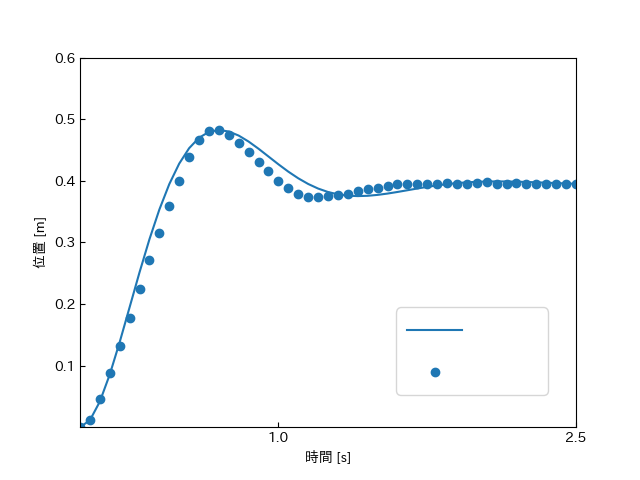
\includegraphics[clip,width=7.0cm]{../img/Initial_MF_doutei.png}
    \caption{M=8.1206,F=34.8243を用いた}
    \label{Initial_MF_doutei}
  \end{center}
\end{figure}
次に,実験データとモデルの時間応答との相対誤差を減らすためにパラメータとして$M$,$F$の改善について考える.
まず,同定実験の結果からステップ応答は振動していることがわかる.まず,$\zeta$について,次式が成り立つ.
\begin{eqnarray}
  \label{MF_zeta}
  \zeta &=& \frac{a_1}{2\omega_n} \nonumber \\
        &=& \frac{F/M}{2\sqrt{a_0}} \nonumber \\
        &=& \frac{F/M}{2\sqrt{\alpha h / M}} \nonumber \\
        &=& \frac{F}{2\sqrt{\alpha h M}}
\end{eqnarray}
そのため,$M$と$F$の関係式について次のことが言える.
\begin{equation}
  \label{MF_F_greater}
  0 < F < 2\sqrt{\alpha h M}
\end{equation}
ここで,$\alpha = 20.09{\rm [N/V]}$,$h = 10{\rm [s]}$を代入すると,次の関係式が得られる.
\begin{equation}
  \label{MF_F_greater_changed}
  0 < F < 20\sqrt{2.009 M}
\end{equation}
この関係式を満たさない範囲では,時間応答は式(\ref{Response_y_t})とならない.
ここで,$M=[4:16]$,$F=[17:36]$の範囲で相対誤差の最小値を求める.
まず$M$の値を2毎にとり,$F$の値を1毎にし,相対誤差のグラフを作る.結果は図\ref{Figure-M=4},\ref{Figure-M=6},\ref{Figure-M=8},\ref{Figure-M=10},\ref{Figure-M=12},\ref{Figure-M=14}となった.
\begin{figure}[H]
  \begin{center}
    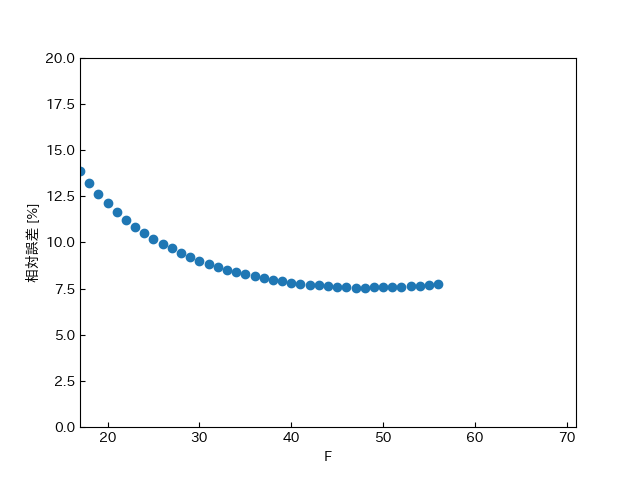
\includegraphics[clip,width=7.0cm]{../img/M-4.png}
    \caption{M=4とした時の相対誤差}
    \label{Figure-M=4}
  \end{center}
\end{figure}
\begin{figure}[H]
  \begin{center}
    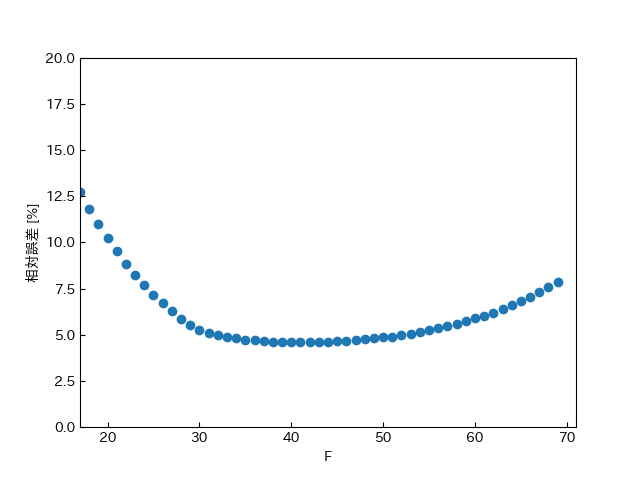
\includegraphics[clip,width=7.0cm]{../img/M-6.png}
    \caption{M=6とした時の相対誤差}
    \label{Figure-M=6}
  \end{center}
\end{figure}
\begin{figure}[H]
  \begin{center}
    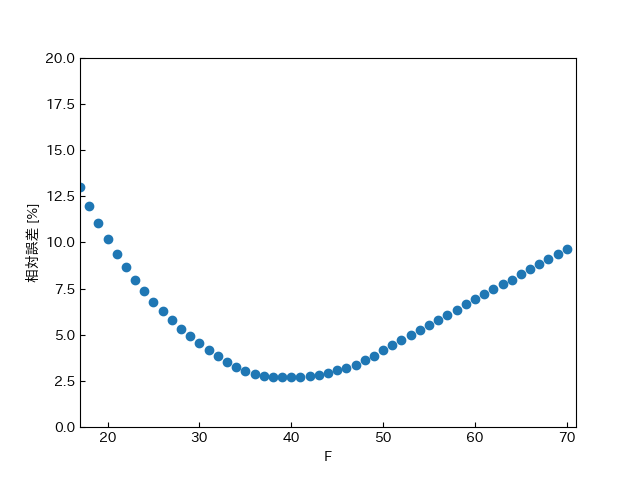
\includegraphics[clip,width=7.0cm]{../img/M-8.png}
    \caption{M=8とした時の相対誤差}
    \label{Figure-M=8}
  \end{center}
\end{figure}
\begin{figure}[H]
  \begin{center}
    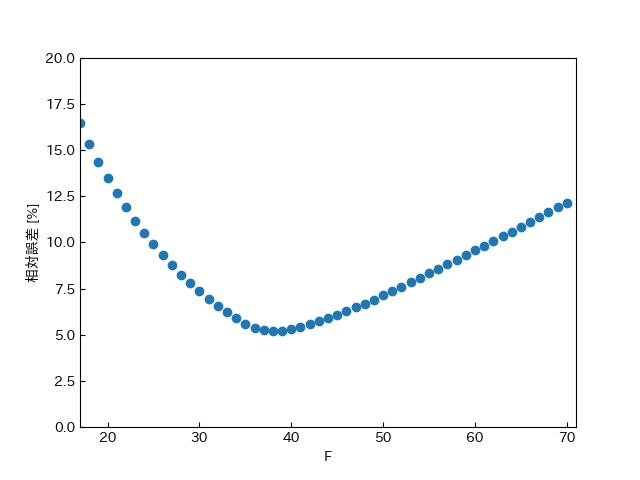
\includegraphics[clip,width=7.0cm]{../img/M-10.png}
    \caption{M=10とした時の相対誤差}
    \label{Figure-M=10}
  \end{center}
\end{figure}
\begin{figure}[H]
  \begin{center}
    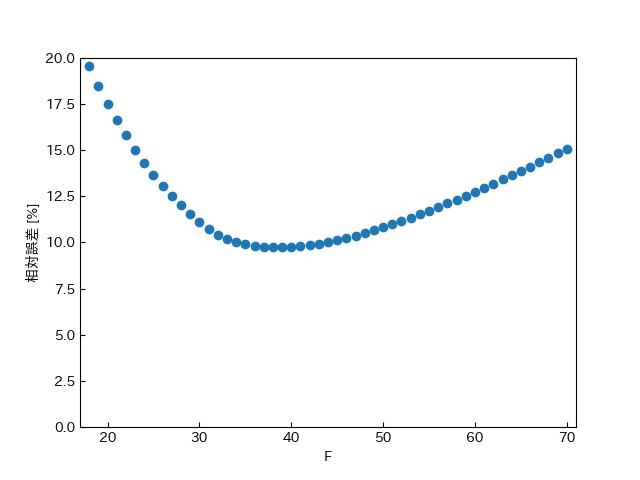
\includegraphics[clip,width=7.0cm]{../img/M-12.png}
    \caption{M=12とした時の相対誤差}
    \label{Figure-M=12}
  \end{center}
\end{figure}
\begin{figure}[H]
  \begin{center}
    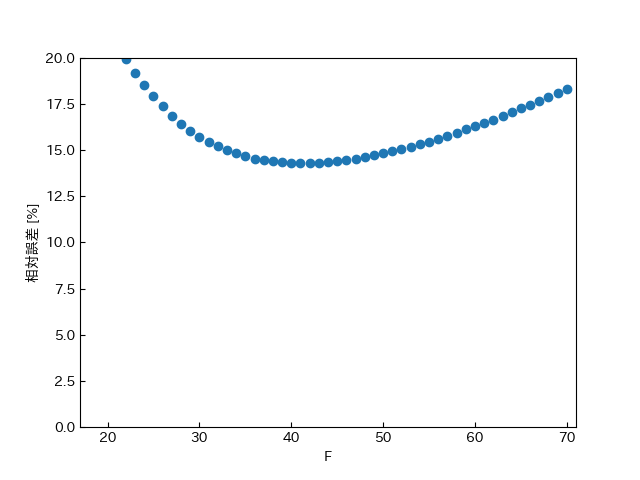
\includegraphics[clip,width=7.0cm]{../img/M-14.png}
    \caption{M=14とした時の相対誤差}
    \label{Figure-M=14}
  \end{center}
\end{figure}
これらのグラフより,$M$,$F$の調べる範囲を改めて,$M=[6:10]$,$F=[30:50]$とし,二分探索により最小の相対誤差を取るように$M$,$F$を決定する.実行したソースコードをソースコード\ref{source_python_MF}に示す.
\newpage
\begin{lstlisting}[caption = python code, label = source_python_MF]
m_left ,m_right = 6, 10
while m_right - m_left>0.0001:
    m_mid = (m_left + m_right)/2
    f_left, f_right = 30, 50
    f_left_score  = modify_MF(t, y, m_mid, f_left)
    f_right_score = modify_MF(t, y, m_mid, f_right)
    while f_right - f_left>0.0001:
        f_mid = (f_left + f_right)/2
        tmp_error = modify_MF(t, y, m_mid, f_mid)
        if f_left_score > f_right_score:
            f_left_score = tmp_error
            f_left = f_mid
        else:
            f_right_score = tmp_error
            f_right = f_mid
    if m_left_score > m_right_score:
        m_left_score = f_left_score
        m_left = m_mid
    else:
        m_right_score = f_left_score
        m_right = m_mid
\end{lstlisting}
結果,$F=40.0001$,$M=7.7496$,相対誤差$2.554[\%]$となった.
この結果を図\ref{Figure-modify_MF_doutei}に示す.
\begin{figure}[tb]
  \begin{center}
    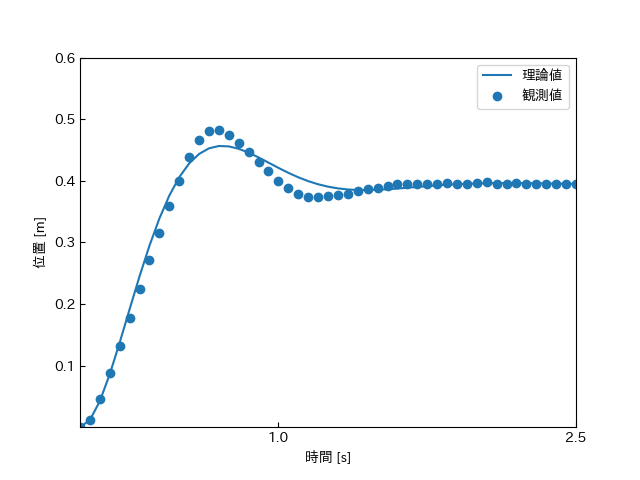
\includegraphics[clip,width=7.0cm]{../img/modify_MF_doute.png}
    \caption{M=7.7496, F=40.0001とした時の応答}
    \label{Figure-modify_MF_doutei}
  \end{center}
\end{figure}
このことにより,状態方程式は次のように表せる.
\begin{equation}
  \label{dotx-Ax+bu}
  \dot{\bm x}(t) = \left[\begin{array}{cc}0&1\\0&-5.1616\end{array}\right]x(t) + \left[\begin{array}{c}0\\2.5924\end{array}\right]u(t)
\end{equation}
フィードバックゲインベクトル$\bm f$,$\bm k$を次のように設定する.
可制御性行列$A_C$は
\begin{equation}
  \label{}
  \bm A_C = \left[\begin{array}{cc}{\bm b} & {\bm A}{\bm b}\end{array}\right]
\end{equation}
である.
不可制御な系では,次式が満たされる.
\begin{equation}
  {\rm det} ({\bm A_C}) = 0
\end{equation}
可観測性行列$A_O$は
\begin{equation}
  \label{}
  \bm A_O = \left[\begin{array}{c}{\bm c}\\{\bm c}{\bm A}\end{array}\right]
\end{equation}である.
不可観測な系では,次式が満たされる.
\begin{equation}
  {\rm det} ({\bm A_O}) = 0
\end{equation}

また状態方程式より特性方程式は
\begin{eqnarray}
  \label{regulator-poll-equation}
  {\rm det}(s{\bm I} - ({\bm A}-{\bm b}{\bm f}))&=&s(s+5.1616+2.5924f_2)+2.5924f_1 \nonumber \\
  &=& s^2 + (5.1616+2.5924f_2)s + 2.5924f_1
\end{eqnarray}
である.
\begin{eqnarray}
  \label{observer-poll-equation}
  {\rm det}(s{\bm I} - ({\bm A}-{\bm K}{\bm c}))&=& (s+k_1)(s+5.1616)+k_2\nonumber \\
  &=& s^2 + (5.1616+k_1)s + (5.1616k_1 + k_2)
\end{eqnarray}
可制御性についての特性多項式は
\begin{equation}
  \label{lambda=-10regletor}
  (s - \lambda_1)(s - \lambda_2)=s^2-(\lambda_1+\lambda_2)s+\lambda_1 \lambda_2
\end{equation}
であり,可観測性についての特性多項式は
\begin{equation}
  \label{lambda=-10observer}
  (s - \lambda_3)(s - \lambda_4)=s^2-(\lambda_3+\lambda_4)s+\lambda_3 \lambda_4
\end{equation}
である.
\begin{description}
  \item[1] 固有値を$\lambda_1=-10$,$\lambda_2=-10$,$\lambda_3=-10$,$\lambda_4=-10$としたもの\\
係数比較により$f_1=38.5743$,$f_2=5.7238$,$k_1=14.8384$,$k_2=23.4101$となる.
  \item[2] 固有値を$\lambda_1=-15$,$\lambda_2=-15$,$\lambda_3=-15$,$\lambda_4=-15$としたもの\\
係数比較により$f_1=86.7922$,$f_2=9.5812$,$k_1=24.8384$,$k_2=96.7941$となる.
  \item[3] 固有値を$\lambda_1=10$,$\lambda_2=10$,$\lambda_3=-10$,$\lambda_4=-10$としたもの\\
係数比較により$f_1=38.5743$,$f_2=5.7238$,$k_1=14.8384$,$k_2=23.4101$となる.
  \item[4] 固有値を$\lambda_1=-10$,$\lambda_2=-10$,$\lambda_3=10$,$\lambda_4=10$としたもの\\
係数比較により$f_1=38.5743$,$f_2=5.7238$,$k_1=14.8384$,$k_2=229.8741$となる.
\end{description}
\section{課題}
\begin{description}
  \item[(1)] 状態量を${\bm z}(t) = \left[\begin{array}{cccc}x_1(t) & x_2(t) & \hat{x}_1(t) & \hat{x}_2(t)\end{array}\right]^T$としたとき,構成した併合系の状態方程式を求めよ.さらに,レギュレータとオブザーバの極の設定に関して考察せよ.
\begin{eqnarray}
  \label{kadai-1}
  {\bm \dot{z}}(t) &=& \left[\begin{array}{cc}{\bm A}&{\bm 0}\\{\bm 0}&{\bm A}\end{array}\right] {\bm z}(t) + \left[\begin{array}{c}{\bm b}\\{\bm b}\end{array}\right] u(t) + \left[\begin{array}{c}{\bm 0}\\{\bm K}\end{array}\right] (y(t) - \hat{y}(t)) \nonumber \\
&=& \left[\begin{array}{cc}{\bm A}&{\bm 0}\\{\bm 0}&{\bm A}\end{array}\right] {\bm z}(t) + \left[\begin{array}{c}{\bm b}\\{\bm b}\end{array}\right] u(t) + \left[\begin{array}{c}{\bm 0}\\{\bm K}\end{array}\right] \left[\begin{array}{cc}{\bm c}{\bm I}&{\bm 0}\\{\bm 0}&-{\bm c}{\bm I}\end{array}\right]{\bm z}(t) \nonumber \\
&=& \left[\begin{array}{cc}{\bm A}&{\bm 0}\\{\bm 0}&{\bm A}-{\bm K}{\bm c}\end{array}\right] {\bm z}(t) + \left[\begin{array}{c}{\bm b}\\{\bm b}\end{array}\right] u(t) \nonumber \\
&=& \left[\begin{array}{cc}{\bm A}&{\bm 0}\\{\bm 0}&{\bm A}-{\bm K}{\bm c}\end{array}\right] {\bm z}(t) - \left[\begin{array}{c}{\bm b}\\{\bm b}\end{array}\right] \left[\begin{array}{cc}{\bm f}&{\bm 0}\end{array}\right]{\bm z}(t) \nonumber \\
&=& \left[\begin{array}{cc}{\bm A}-{\bm b}{\bm f}&{\bm 0}\\-{\bm b}{\bm f}&{\bm A}-{\bm K}{\bm c}\end{array}\right] {\bm z}(t)
\end{eqnarray}
  \item[(2)] 制御結果について考察し,収束速度を上げる.過渡応答の振動を抑える,もしくは入力量を抑えるような結果を得るためには,制御系をどのように改良すればよいか検討せよ.
\end{description}
\end{document}
